\documentclass[11pt,notitlepage]{article}

\usepackage[comma,numbers,sort&compress]{natbib}
\usepackage{graphicx}
\usepackage{color}
\usepackage{soul}
\usepackage{amssymb}
\usepackage{amsbsy}
\usepackage{theorem}
\usepackage{xcolor}
\usepackage{fullpage}
\usepackage{amsmath}
\usepackage{bm}
\usepackage{empheq}
\usepackage{centernot}
\usepackage{mathtools}
\usepackage{stmaryrd}
\usepackage[margin=1cm]{caption}
\usepackage{algorithmic}
\usepackage{helvet}
\renewcommand{\familydefault}{\sfdefault}
\usepackage[affil-it]{authblk}

\begin{document}

\section{Summary vision statement}
\begin{enumerate}
 \item Core methodology:
        \begin{enumerate}
        \item  NLP parsing
        \item  1st order probabilistic logic
        \item modified Dijkstra
        \item other probabilistic data analysis approaches?
  		\end{enumerate}
 \item Limitations addressed:
        \begin{enumerate}
        \item No incorporation of uncertainty in all steps of the process
        \item inability to use natural language queries
        \item inability to automate identification of relevant knowledge sources
        \item inability to automate the selection of relevant queries
        \end{enumerate}
 \item Expertise:
 		\begin{enumerate}
        \item Steve and Liang will have to put there expertise in here
        Mine is: mathematical algorithms for fast approximate or exact analysis of big data problems (can give references)
        \end{enumerate}
 \item Previous applications:
 		\begin{enumerate}
        \item Autonomous service robots (10.1177/0278364913481635),
        \item IBM Watson is also based off of probabilistic evidence-based architecture (Magazine, A. I. "The ai behind watson—the technical article." AI Magazine (2010).)
        \item Suggested for use with precision oncology (10.1038/nrclinonc.2013.244)
        \item Similar approaches in drug-target interaction prediction (10.1109/TCBB.2014.2325031)
        \item Liang, more accurate previous applications?
        \end{enumerate}
\end{enumerate}

\subsection{Limitations and bottlenecks in the current state of the art}

\section{Project plan}
\subsection{Overview of methodology to be used}
The methodology we propose to autonomously answer user queries consists of three main components: process natural language user queries, generate a dossier of search strategies, and execute the desired search strategies.
\subsection{Natural language processing}
\label{section:NLP}
A critical functionality of a reasoning engine is the ability to parse and understand free-form user input. To facilitate this, we...
\textbf{Liang's NLP paragraph here}
The NLP step will result in ... This representation of the user query will be used by the reasoning engine to generate a dossier of search strategies. 
%an identification of relevant abstract terms (such as ``disease,'' ``pathway,'', ``molecule'' etc.) along with a desired connectives between them (such as ``offers protection against,'' ``is associated to'' etc.).
\subsection{Generate a dossier of search strategies}
\label{section:strategies}
Our Reasoning Engine will simultaneously identify relevant knowledge sources and construct appropriate queries in order to answer user questions. This is accomplished by constructing a network of \textit{schemas} and other metadata of Knowledge Sources (KS's) which we call a \textit{schema network}. This representation will not be a network of all biological interactions and entities contained in the KS's, but rather compactly and abstractly represents the categories of information contained in the various Translator KS's as well as the relationships between them. Using the parsed user input, our Reasoning Engine will identify appropriate paths in this network that represent search strategies to answer the user query. These paths will traverse one or more KS's metadata and hence will automatically identify the relevant databases to query. To find such paths, we will implement a reasoning engine based on the formalism of Tractable First-Order Probabilistic Logic and its associated Tractable Markov Logic (TML) language developed by \citet{Domingos:2012wi}. The Java-based (and open-source) NCATS-Tangerine Beacon Aggregator is used to obtain metadata (schemas and entity counts) from Knowledge Sources via RESTful queries leveraging the common Translator Knowledge Beacon Application Programming Interface (KBAPI). This provides the topology of the schema network. 

\textbf{Training?}

%\subsubsection{Tractable Markov Logic}
%In keeping with the distributed nature of Translator's Knowledge Sources, the reasoning engine that will generate the dossier will operate on a Markov Logic Network learned from the {\em schemas\/} and other metdata of Knowledge Sources; it will not be a network of all biological interactions contained in the Knowledge Sources. The reasoning engine's input will be a data structure representing the parsed natural language query (see Sec.~\ref{sec:nlp}). The reasoning engine's output will be a {\em dossier,\/} i.e., a ranked list of {\em search strategies,\/} where a search strategy is a possible joining of result-sets from one or more queries of Translator Knowledge Sources (KS).

\subsubsection{Example to show how the reasoning engine will work}
We will illustrate the {\em dossier generation\/} idea with a concrete example. Suppose a user wishes to find a common mechanism to explain the association of a variant $V$ with two different diseases $D1$ and $D2$ (Fig.~\ref{fig:networks}a).
\begin{figure}[h!]
  \begin{tabular}{cccc}
    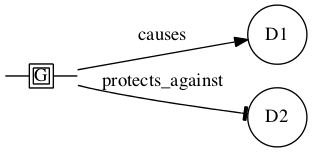
\includegraphics[width=1.4in]{baseproblem.png} &
    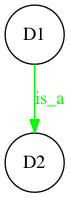
\includegraphics[width=0.35in]{net1.png} &
    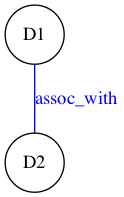
\includegraphics[width=0.6in]{net2.png} &
    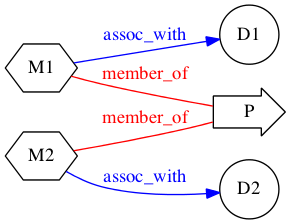
\includegraphics[width=1.5in]{net3.png}\\
    {\bf (a) Query} & {\bf (b) Search Strategy 1} & {\bf (c) Search Strategy 2} & {\bf (d) Search Strategy 3}
  \end{tabular}
  \caption{Example query predicate information (A) and examples of possible search strategies (B--D) that would be examined by the reasoning engine based on a Markov Logic Network representing possible {\em types of connections\/}  between relevant biological entities. Color denotes database to be searched (green: Disease Ontology, blue: DisGeNET, red: Pathway Commons). Black edges denote the query predicate variant-disease relationships. Circles denote the diseases D1 and D2, the boxed G denotes a variant, the large arrow shape denotes a pathway P, and hexagons denote the protein molecules M1 and M2 (or equivalently, their associated genes).}
  \label{fig:networks}
\end{figure}
The goal will be to find paths in the schema network that describe common mechanisms between the input diseases. One possible kind of path is a (disease,disease) tuple representing ``is a subtype of'' relationships (Fig.~\ref{fig:networks}b). This kind of relationship between diseases is inferred from the metadata of the Gene Ontology database. An alternate path consists of a undirected edges $\{$disease,disease$\}$ representing disease-disease associations from the DisGeNET database (Fig.~\ref{fig:networks}c). A more complicated path (traversing two different databases) is given in Fig.~\ref{fig:networks}b) where  (molecule,disease) ``associated\_with'' tuples (from DisGeNET or Pharos) with (molecule,pathway) tuples representing ``member\_of'' relationships from Pathway Commons. An example of a {\em three}-database search strategy, for the same user query (Fig.~\ref{fig:threedb}a) about a variant-to-two-diseases association, is shown in Fig.~\ref{fig:threedb}b).

Each of these possible paths identifies relevant KS's and represents a search strategy: how to traverse these databases to answer the user query. A na\''ive approach to ranking these different search strategies would be to use a combination of path length with edge weightings based on, say, prevalence of the given diseases $D1$ and $D2$,  strength of associations, etc. A more nuanced approach is to utilize the TML language \citet{Domingos:2012wi} to rank the search strategies in terms of how well they answer the user input. After the user selects a desired search strategy (alternatively, the top ranked search strategy is automatically utilized), the source and target nodes are grounded with the particular biological entities contained in the user query. A modified Dijkstra algorithm (Section \ref{section:Dijkstra}) is then used to execute the query on the databases of interest to find paths between actual biological entities.

%The schema network contains many different kinds of paths between a The schema network will contain various paths between the disease label and itself. For example, one such path is $D1$ ``is a``

%A simple strategy would be to search to obtain a list of (disease,disease) tuples representing ``is-a'' relationships from the Gene Ontology database (Fig.~\ref{fig:networks}b) where the edge would be assigned a weight in the Markov Logic Network based on the strength of evidence of this information type (either a fixed weight for the database, or with more information, the weight could be the ratio of prevalence of $D1$ to prevalence of $D2$). (We note that this search strategy would not be selected by the reasoning engine because the ``is a'' relationship between two diseases is not consistent with the variant being protective against disease D2 and causal for disease D1). An alternative simple search strategy would be to load a list of {\em undirected\/} $\{$disease,disease$\}$ pairs representing disease-disease associations from the DisGeNET database (Fig.~\ref{fig:networks}c). An example of a {\em two}-database search strategy would be to join (molecule,disease) ``associated\_with'' tuples (from DisGeNET or Pharos) with (molecule,pathway) tuples representing ``member\_of'' relationships from Pathway Commons (Fig.~\ref{fig:networks}d). An example of a {\em three}-database search strategy, for the same user query about a variant-to-two-diseases association (Fig.~\ref{fig:threedb}a), is shown in Fig.~\ref{fig:threedb}b.
\begin{figure}[h!]
  \begin{tabular}{ccc}
  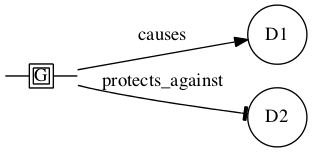
\includegraphics[width=1.4in]{baseproblem.png} &    
  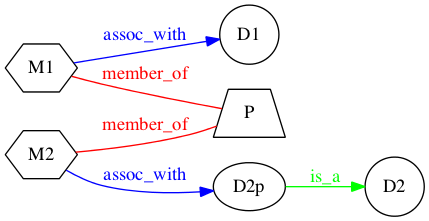
\includegraphics[width=2in]{net4.png} &
  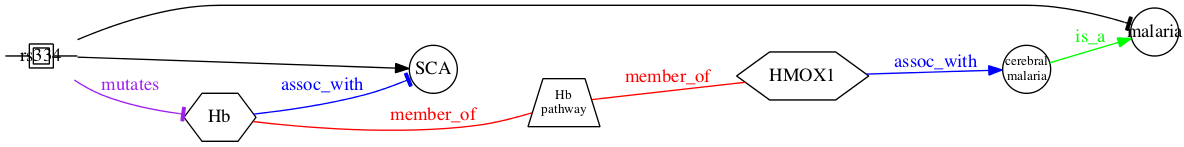
\includegraphics[width=2.5in]{net5.png} \\
                  {\bf (a) Query} & {\bf (b) Search Strategy 4} & {\bf (c) Search Result}
  \end{tabular}
  \caption{Example query predicate information (A); three-database example search strategy (B); matching search result for the specific query example G=rs334, D1=sicke-cell anemia (SCA) and D2=malaria (C). Edge color denotes the Knowledge Source to be searched (blue, DisGeNET; red, Pathway Commons; and green, Disease Ontology). Black edges denote the original query. Purple edge is the inferred interaction that explains the two black edges in light of the colored edges.}
  \label{fig:threedb}
\end{figure}
As an example, assume that the variant G in this example query scenario is rs334, a pleiotropic rare (MAF = 0.014\%) variant for which the homozygous minor allele causes the blood disorder sickle-cell anemia (D1) and protects against malaria (D2). A Dijkstra search on the three-database search strategy shown in Fig.~\ref{fig:threedb}b) would yield a match indicating that a potential explanation for the pleiotropy of rs334 is that it inhibits the hemoglobin pathway, thus reducing circulating levels of free heme, which has been reported to be protective in the case of cerebral malaria (a neurological complication of malarial disease)~\cite{Ferreira:2011ff}.

\subsection{Executing search strategies}
\label{section:Dijkstra}
After the search strategy (path through the schema network) is selected, we employ a modified Dijkstra algorithm to find probable paths between source and target node(s).
\textbf{Steve, Liang, insert description here}

%\subsubsection{Composition of the Markov Logic Network}
%We will use the Java-baesd (and open-source) NCATS-Tangerine Beacon Aggregator to obtain metadata (schemas and entity counts) from Knowledge Sources via RESTful queries leveraging the common Translator Knowledge Beacon Application Programming Interface (KBAPI).


\subsection{Anticipated functionality for the POC reasoning tool}
For the two proof of concept project questions, the anticipated functionality includes:
\begin{enumerate}
\item Allow the user to select from one of two questions (``which genetic condition(s) protect(s) from a given disease $D$'' and ``what is the outcome pathway for drug $D$ and condition $C$'') where $D$ and $C$ are drugs and conditions that can be specified by the user.
\item Pre-computed search strategies for these two questions will be implemented.
\item The modified Dijkstra algorithm will be implemented and will query the Knowledge Sources in real time (based on the user selected search query)
\end{enumerate}
If funded, the Reasoning Engine we propose will allow for natural language input (Section \ref{section:NLP}), automatic generation of search strategies (Section \ref{section:strategies}) and will also utilize the Dijkstra algorithm of Section \ref{section:Dijkstra}
\textit{Functionality for the reasoning tool proof-of-concept (due in Nov)}
\subsection{Components of the proposed software stack}


%\subsubsection{Natural language query analyzer}
%\label{sec:nlp}
%Should we use the Stanford CoreNLP with BioNLP shared task data? If so, which Python API should we use? (There are about a dozen of them).

\subsection{How proposed software will interact with Translator}

%% \section{Background: Types of questions}
%% \subsection{How does drug X induce clinical outcome Y?}
%% \subsection{Why do variants that cause sicke-cell anemia protect against malaria?}
%% \subsection{In people with variants found in any of the 22 known FA genes, is there increasing incidence of apalastic anemia
%%   (or other diseases)?}
%% \subsection{What venomous species have resulted in drugs approved by the FDA?}
%% \subsection{What cellular processes in which tissues are impacted in a patient-based EMR?}
%% \subsection{Why does ingestion of GlcNAc ameliorate symptoms of ngly1 deficiency?}

%% \section{Background: Knowledge Sources}
%% \begin{description}
%% \item[EBI String]{Protein-protein interactions}
%% \end{description}

\section{Personnel}

\bibliographystyle{plainnat}
\bibliography{conclett}

\end{document}
